\documentclass[twoside]{book}

% Packages required by doxygen
\usepackage{fixltx2e}
\usepackage{calc}
\usepackage{doxygen}
\usepackage[export]{adjustbox} % also loads graphicx
\usepackage{graphicx}
\usepackage[utf8]{inputenc}
\usepackage{makeidx}
\usepackage{multicol}
\usepackage{multirow}
\PassOptionsToPackage{warn}{textcomp}
\usepackage{textcomp}
\usepackage[nointegrals]{wasysym}
\usepackage[table]{xcolor}

% Font selection
\usepackage[T1]{fontenc}
\usepackage[scaled=.90]{helvet}
\usepackage{courier}
\usepackage{amssymb}
\usepackage{sectsty}
\renewcommand{\familydefault}{\sfdefault}
\allsectionsfont{%
  \fontseries{bc}\selectfont%
  \color{darkgray}%
}
\renewcommand{\DoxyLabelFont}{%
  \fontseries{bc}\selectfont%
  \color{darkgray}%
}
\newcommand{\+}{\discretionary{\mbox{\scriptsize$\hookleftarrow$}}{}{}}

% Page & text layout
\usepackage{geometry}
\geometry{%
  a4paper,%
  top=2.5cm,%
  bottom=2.5cm,%
  left=2.5cm,%
  right=2.5cm%
}
\tolerance=750
\hfuzz=15pt
\hbadness=750
\setlength{\emergencystretch}{15pt}
\setlength{\parindent}{0cm}
\setlength{\parskip}{3ex plus 2ex minus 2ex}
\makeatletter
\renewcommand{\paragraph}{%
  \@startsection{paragraph}{4}{0ex}{-1.0ex}{1.0ex}{%
    \normalfont\normalsize\bfseries\SS@parafont%
  }%
}
\renewcommand{\subparagraph}{%
  \@startsection{subparagraph}{5}{0ex}{-1.0ex}{1.0ex}{%
    \normalfont\normalsize\bfseries\SS@subparafont%
  }%
}
\makeatother

% Headers & footers
\usepackage{fancyhdr}
\pagestyle{fancyplain}
\fancyhead[LE]{\fancyplain{}{\bfseries\thepage}}
\fancyhead[CE]{\fancyplain{}{}}
\fancyhead[RE]{\fancyplain{}{\bfseries\leftmark}}
\fancyhead[LO]{\fancyplain{}{\bfseries\rightmark}}
\fancyhead[CO]{\fancyplain{}{}}
\fancyhead[RO]{\fancyplain{}{\bfseries\thepage}}
\fancyfoot[LE]{\fancyplain{}{}}
\fancyfoot[CE]{\fancyplain{}{}}
\fancyfoot[RE]{\fancyplain{}{\bfseries\scriptsize Generated by Doxygen }}
\fancyfoot[LO]{\fancyplain{}{\bfseries\scriptsize Generated by Doxygen }}
\fancyfoot[CO]{\fancyplain{}{}}
\fancyfoot[RO]{\fancyplain{}{}}
\renewcommand{\footrulewidth}{0.4pt}
\renewcommand{\chaptermark}[1]{%
  \markboth{#1}{}%
}
\renewcommand{\sectionmark}[1]{%
  \markright{\thesection\ #1}%
}

% Indices & bibliography
\usepackage{natbib}
\usepackage[titles]{tocloft}
\setcounter{tocdepth}{3}
\setcounter{secnumdepth}{5}
\makeindex

% Custom commands
\newcommand{\clearemptydoublepage}{%
  \newpage{\pagestyle{empty}\cleardoublepage}%
}

\usepackage{caption}
\captionsetup{labelsep=space,justification=centering,font={bf},singlelinecheck=off,skip=4pt,position=top}

%===== C O N T E N T S =====

\begin{document}

% Titlepage & ToC
\pagenumbering{alph}
\begin{titlepage}
\vspace*{7cm}
\begin{center}%
{\Large A\+P\+EX }\\
\vspace*{1cm}
{\large Generated by Doxygen 1.8.13}\\
\end{center}
\end{titlepage}
\clearemptydoublepage
\pagenumbering{roman}
\tableofcontents
\clearemptydoublepage
\pagenumbering{arabic}

%--- Begin generated contents ---
\chapter{Hierarchical Index}
\section{Class Hierarchy}
This inheritance list is sorted roughly, but not completely, alphabetically\+:\begin{DoxyCompactList}
\item \contentsline{section}{A\+P\+E\+X\+Dependency\+Function}{\pageref{structAPEXDependencyFunction}}{}
\item \contentsline{section}{A\+P\+E\+X\+Dependency\+Graph}{\pageref{structAPEXDependencyGraph}}{}
\item \contentsline{section}{A\+P\+E\+X\+Dependency\+Node}{\pageref{structAPEXDependencyNode}}{}
\item Module\+Pass\begin{DoxyCompactList}
\item \contentsline{section}{A\+P\+E\+X\+Pass}{\pageref{classAPEXPass}}{}
\end{DoxyCompactList}
\end{DoxyCompactList}

\chapter{Data Structure Index}
\section{Data Structures}
Here are the data structures with brief descriptions\+:\begin{DoxyCompactList}
\item\contentsline{section}{\textbf{ A\+P\+E\+X\+Dependency\+Function} \\*Function (can contain multiple basic blocks) }{\pageref{structAPEXDependencyFunction}}{}
\item\contentsline{section}{\textbf{ A\+P\+E\+X\+Dependency\+Graph} \\*Graph\+: consists of nodes that are functions }{\pageref{structAPEXDependencyGraph}}{}
\item\contentsline{section}{\textbf{ A\+P\+E\+X\+Dependency\+Node} \\*Node is usually line instruction of IR. Sometimes whole function }{\pageref{structAPEXDependencyNode}}{}
\item\contentsline{section}{\textbf{ A\+P\+E\+X\+Pass} \\*Actual A\+P\+EX pass }{\pageref{classAPEXPass}}{}
\end{DoxyCompactList}

\chapter{Data Structure Documentation}
\section{A\+P\+E\+X\+Dependency\+Function Struct Reference}
\label{structAPEXDependencyFunction}\index{A\+P\+E\+X\+Dependency\+Function@{A\+P\+E\+X\+Dependency\+Function}}


Function (can contain multiple basic blocks).  




{\ttfamily \#include $<$apex.\+h$>$}

\subsection*{Data Fields}
\begin{DoxyCompactItemize}
\item 
\mbox{\label{structAPEXDependencyFunction_ad40a9b218b3412fbef6d251c096348da}} 
Value $\ast$ {\bfseries value}
\item 
\mbox{\label{structAPEXDependencyFunction_a88b9c8546d91814c01326726b91b882a}} 
std\+::vector$<$ \textbf{ A\+P\+E\+X\+Dependency\+Node} $>$ {\bfseries nodes}
\end{DoxyCompactItemize}


\subsection{Detailed Description}
Function (can contain multiple basic blocks). 

Definition at line 40 of file apex.\+h.



The documentation for this struct was generated from the following file\+:\begin{DoxyCompactItemize}
\item 
apex.\+h\end{DoxyCompactItemize}

\section{A\+P\+E\+X\+Dependency\+Graph Struct Reference}
\label{structAPEXDependencyGraph}\index{A\+P\+E\+X\+Dependency\+Graph@{A\+P\+E\+X\+Dependency\+Graph}}


Graph\+: consists of nodes that are functions.  




{\ttfamily \#include $<$apex.\+h$>$}

\subsection*{Data Fields}
\begin{DoxyCompactItemize}
\item 
\mbox{\label{structAPEXDependencyGraph_ab358b0afe44dc73e8db4c53689de6aa8}} 
std\+::vector$<$ \textbf{ A\+P\+E\+X\+Dependency\+Function} $>$ {\bfseries functions}
\item 
\mbox{\label{structAPEXDependencyGraph_af6237ef27a89f712d5fe205f9052c31f}} 
std\+::map$<$ L\+L\+V\+M\+Node $\ast$, std\+::vector$<$ L\+L\+V\+M\+Node $\ast$ $>$ $>$ {\bfseries node\+\_\+data\+\_\+dependencies\+\_\+map}
\item 
\mbox{\label{structAPEXDependencyGraph_a582babaf3ee3b4c17c347d1c2917515d}} 
std\+::map$<$ L\+L\+V\+M\+Node $\ast$, \textbf{ A\+P\+E\+X\+Dependency\+Function} $\ast$ $>$ {\bfseries node\+\_\+function\+\_\+map}
\end{DoxyCompactItemize}


\subsection{Detailed Description}
Graph\+: consists of nodes that are functions. 

Definition at line 48 of file apex.\+h.



The documentation for this struct was generated from the following file\+:\begin{DoxyCompactItemize}
\item 
apex.\+h\end{DoxyCompactItemize}

\section{A\+P\+E\+X\+Dependency\+Node Struct Reference}
\label{structAPEXDependencyNode}\index{A\+P\+E\+X\+Dependency\+Node@{A\+P\+E\+X\+Dependency\+Node}}


Node is usually line instruction of IR. Sometimes whole function.  




{\ttfamily \#include $<$apex.\+h$>$}

\subsection*{Data Fields}
\begin{DoxyCompactItemize}
\item 
\mbox{\label{structAPEXDependencyNode_a970e7a2fef904e104bff4c2fc5ff2cb1}} 
L\+L\+V\+M\+Node $\ast$ {\bfseries node}
\item 
\mbox{\label{structAPEXDependencyNode_a8b3b641572bf365c4f731fc83b169984}} 
Value $\ast$ {\bfseries value}
\item 
\mbox{\label{structAPEXDependencyNode_a6c402ac3d515fb024c9d8e08aced4f5c}} 
std\+::vector$<$ L\+L\+V\+M\+Node $\ast$ $>$ {\bfseries control\+\_\+depenencies}
\item 
\mbox{\label{structAPEXDependencyNode_ae526db6103f708c8cfacbb0af242c65f}} 
std\+::vector$<$ L\+L\+V\+M\+Node $\ast$ $>$ {\bfseries rev\+\_\+control\+\_\+depenencies}
\item 
\mbox{\label{structAPEXDependencyNode_ade99c6315545e206d562789348540cc0}} 
std\+::vector$<$ L\+L\+V\+M\+Node $\ast$ $>$ {\bfseries data\+\_\+dependencies}
\item 
\mbox{\label{structAPEXDependencyNode_abcf07bec655009d666e6f2c1163f4dcb}} 
std\+::vector$<$ L\+L\+V\+M\+Node $\ast$ $>$ {\bfseries rev\+\_\+data\+\_\+dependencies}
\end{DoxyCompactItemize}


\subsection{Detailed Description}
Node is usually line instruction of IR. Sometimes whole function. 

Definition at line 30 of file apex.\+h.



The documentation for this struct was generated from the following file\+:\begin{DoxyCompactItemize}
\item 
apex.\+h\end{DoxyCompactItemize}

\section{A\+P\+E\+X\+Pass Class Reference}
\label{classAPEXPass}\index{A\+P\+E\+X\+Pass@{A\+P\+E\+X\+Pass}}


Actual A\+P\+EX pass.  




{\ttfamily \#include $<$apex.\+h$>$}

Inheritance diagram for A\+P\+E\+X\+Pass\+:\begin{figure}[H]
\begin{center}
\leavevmode
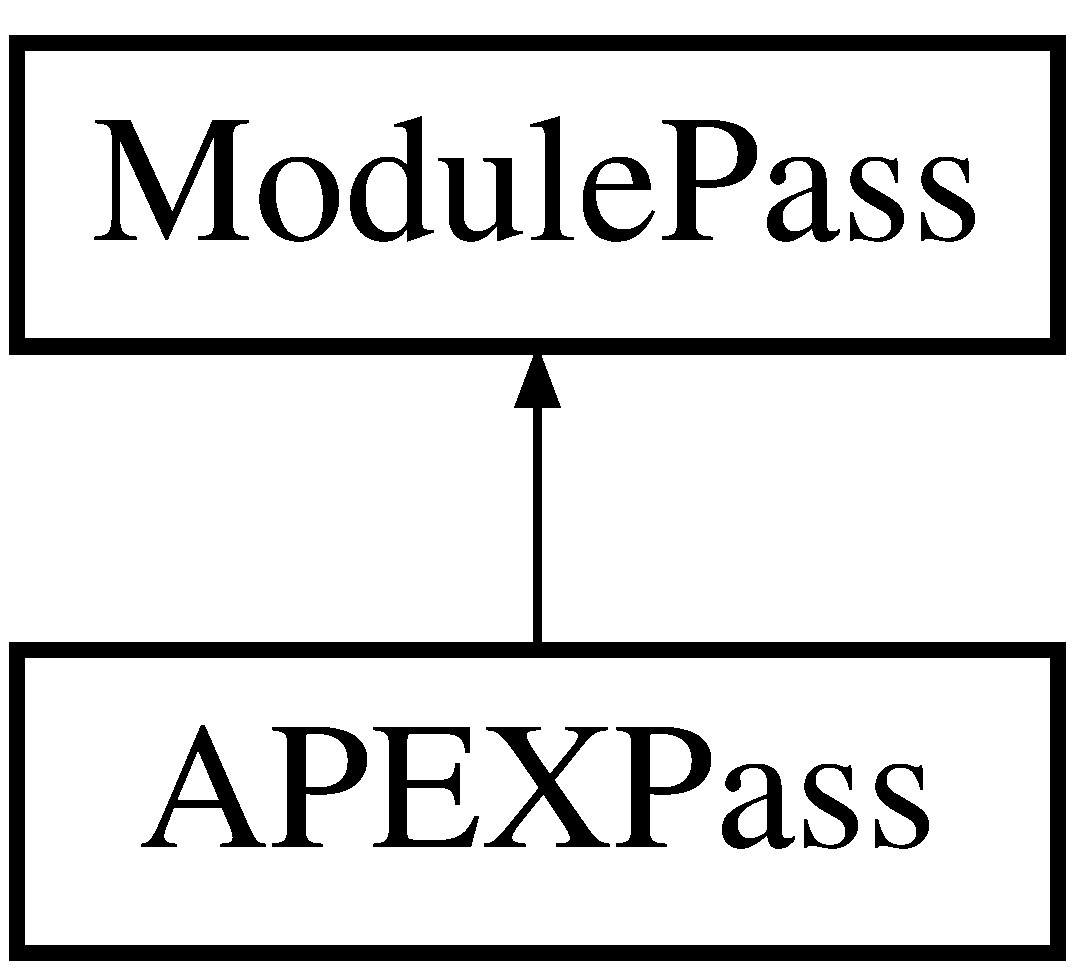
\includegraphics[height=2.000000cm]{classAPEXPass}
\end{center}
\end{figure}
\subsection*{Public Member Functions}
\begin{DoxyCompactItemize}
\item 
\mbox{\label{classAPEXPass_a66542ebffe823d7b5deea34a34fb8c4e}} 
bool \textbf{ run\+On\+Module} (Module \&M) override
\begin{DoxyCompactList}\small\item\em Running on each module. \end{DoxyCompactList}\end{DoxyCompactItemize}
\subsection*{Static Public Attributes}
\begin{DoxyCompactItemize}
\item 
\mbox{\label{classAPEXPass_a5811ea00952c46c1ee459f4ed39d48fa}} 
static char \textbf{ ID} = 0
\begin{DoxyCompactList}\small\item\em Registering our own pass, so it can be ran via opt. \end{DoxyCompactList}\end{DoxyCompactItemize}
\subsection*{Private Member Functions}
\begin{DoxyCompactItemize}
\item 
\mbox{\label{classAPEXPass_a8a597daae8f501ccf5dbf9bb2a147a09}} 
void \textbf{ log\+Print} (const std\+::string \&message)
\begin{DoxyCompactList}\small\item\em Simple logging print with newline. \end{DoxyCompactList}\item 
\mbox{\label{classAPEXPass_a6d149e003989eee09bf7b13db230434e}} 
void \textbf{ log\+Print\+Underline} (const std\+::string \&message)
\begin{DoxyCompactList}\small\item\em Simple logging print with newline. \end{DoxyCompactList}\item 
\mbox{\label{classAPEXPass_adc29fc0e46c7d6d8d776cea43f15e8cc}} 
void \textbf{ log\+Print\+Flat} (const std\+::string \&message)
\begin{DoxyCompactList}\small\item\em Simple logging print W\+I\+T\+H\+O\+UT newline. \end{DoxyCompactList}\item 
\mbox{\label{classAPEXPass_abc646851a9b4be4892d03a8f5226ff24}} 
void \textbf{ log\+Dump\+Module} (const Module \&M)
\begin{DoxyCompactList}\small\item\em Dumps whole module M. \end{DoxyCompactList}\item 
\mbox{\label{classAPEXPass_a9712ed455068d007517c3a68d4e3a72c}} 
void \textbf{ function\+Vector\+Flat\+Print} (const std\+::vector$<$ Function $\ast$$>$ \&functions)
\begin{DoxyCompactList}\small\item\em Prints contents of the vector functions. \end{DoxyCompactList}\item 
int \textbf{ function\+Remove\+Calls} (const Function $\ast$F)
\begin{DoxyCompactList}\small\item\em Takes pointer to function F, iterates over instructions calling this function and removes these instructions. \end{DoxyCompactList}\item 
int \textbf{ function\+Remove} (Function $\ast$F)
\begin{DoxyCompactList}\small\item\em Takes pointer to a function F, removes all calls to this function and then removes function F itself. \end{DoxyCompactList}\item 
int \textbf{ function\+Get\+Callers} (const Function $\ast$F, std\+::vector$<$ Function $\ast$$>$ \&callers)
\begin{DoxyCompactList}\small\item\em Collects functions that call function F into vector callers. \end{DoxyCompactList}\item 
int \textbf{ function\+Get\+Callees} (const Function $\ast$F, std\+::vector$<$ Function $\ast$$>$ \&callees)
\begin{DoxyCompactList}\small\item\em Collects functions that are called by function F into vector callees. \end{DoxyCompactList}\item 
int \textbf{ create\+Call\+Graph} (const Module \&M, const std\+::string \&root, std\+::vector$<$ std\+::pair$<$ Function $\ast$, std\+::vector$<$ Function $\ast$$>$$>$$>$ \&callgraph)
\begin{DoxyCompactList}\small\item\em Creates callgraph from module M, starting from the function with global id specified in root. \end{DoxyCompactList}\item 
\mbox{\label{classAPEXPass_a9022380512661408b24f1351a0e72a65}} 
void \textbf{ print\+Call\+Graph} (const std\+::vector$<$ std\+::pair$<$ Function $\ast$, std\+::vector$<$ Function $\ast$$>$$>$$>$ \&callgraph)
\begin{DoxyCompactList}\small\item\em Prints callgraph. \end{DoxyCompactList}\item 
int \textbf{ find\+Path} (const std\+::vector$<$ std\+::pair$<$ Function $\ast$, std\+::vector$<$ Function $\ast$$>$$>$$>$ \&callgraph, const std\+::string \&source, const std\+::string \&target, std\+::vector$<$ Function $\ast$$>$ \&final\+\_\+path)
\begin{DoxyCompactList}\small\item\em Uses B\+FS to find path in callgraph from source to target (both are global Function I\+Ds). \end{DoxyCompactList}\item 
\mbox{\label{classAPEXPass_aecb2f67cbbfc8622aaf1e7b4b141995d}} 
void \textbf{ print\+Path} (const std\+::vector$<$ Function $\ast$$>$ \&path, const std\+::string \&source, const std\+::string \&target)
\begin{DoxyCompactList}\small\item\em Prints path. \end{DoxyCompactList}\item 
\mbox{\label{classAPEXPass_a960948a62a5a07ac11caaaf3de4ceb77}} 
void \textbf{ dg\+Init} (Module \&M, L\+L\+V\+M\+Dependence\+Graph \&dg)
\begin{DoxyCompactList}\small\item\em Initializes dg and calculates control \& data dependencies. \end{DoxyCompactList}\item 
void \textbf{ apex\+Dg\+Init} (\textbf{ A\+P\+E\+X\+Dependency\+Graph} \&apex\+\_\+dg)
\begin{DoxyCompactList}\small\item\em Extracts data from dg and stores them into apex\+\_\+dg structure. \end{DoxyCompactList}\item 
void \textbf{ apex\+Dg\+Get\+Block\+Node\+Info} (\textbf{ A\+P\+E\+X\+Dependency\+Node} \&apex\+\_\+node, L\+L\+V\+M\+Node $\ast$node)
\begin{DoxyCompactList}\small\item\em Stores control/reverse\+\_\+control/data/reverse\+\_\+data dependencies of the node to the apex\+\_\+node. \end{DoxyCompactList}\item 
\mbox{\label{classAPEXPass_a643d4916f69e20006c14396bec4b16fe}} 
void \textbf{ apex\+Dg\+Print} (\textbf{ A\+P\+E\+X\+Dependency\+Graph} \&apex\+\_\+dg, bool verbose)
\begin{DoxyCompactList}\small\item\em Pretty prints \doxyref{A\+P\+E\+X\+Dependency\+Graph}{p.}{structAPEXDependencyGraph} structure. \end{DoxyCompactList}\item 
\mbox{\label{classAPEXPass_ad6dfc083ac1a01b0224af4ae6b69163e}} 
void \textbf{ apex\+Dg\+Print\+Data\+Dependenies\+Compact} (\textbf{ A\+P\+E\+X\+Dependency\+Graph} \&apex\+\_\+dg)
\begin{DoxyCompactList}\small\item\em Pretty prints apex\+\_\+dg, but only with data dependencies. \end{DoxyCompactList}\item 
void \textbf{ apex\+Dg\+Make\+Graph\+Print} (\textbf{ A\+P\+E\+X\+Dependency\+Graph} \&apex\+\_\+dg, bool print\+\_\+graph)
\begin{DoxyCompactList}\small\item\em Takes apex\+\_\+dg, makes graph out of data dependencies between nodes and stores this graph into apex\+\_\+dg.\+graph variable. \end{DoxyCompactList}\end{DoxyCompactItemize}


\subsection{Detailed Description}
Actual A\+P\+EX pass. 

Definition at line 56 of file apex.\+h.



\subsection{Member Function Documentation}
\mbox{\label{classAPEXPass_a792707395fe9ebea89abcfcf8bd00067}} 
\index{A\+P\+E\+X\+Pass@{A\+P\+E\+X\+Pass}!apex\+Dg\+Get\+Block\+Node\+Info@{apex\+Dg\+Get\+Block\+Node\+Info}}
\index{apex\+Dg\+Get\+Block\+Node\+Info@{apex\+Dg\+Get\+Block\+Node\+Info}!A\+P\+E\+X\+Pass@{A\+P\+E\+X\+Pass}}
\subsubsection{apex\+Dg\+Get\+Block\+Node\+Info()}
{\footnotesize\ttfamily void A\+P\+E\+X\+Pass\+::apex\+Dg\+Get\+Block\+Node\+Info (\begin{DoxyParamCaption}\item[{\textbf{ A\+P\+E\+X\+Dependency\+Node} \&}]{apex\+\_\+node,  }\item[{L\+L\+V\+M\+Node $\ast$}]{node }\end{DoxyParamCaption})\hspace{0.3cm}{\ttfamily [private]}}



Stores control/reverse\+\_\+control/data/reverse\+\_\+data dependencies of the node to the apex\+\_\+node. 



Definition at line 490 of file apex.\+cpp.



Referenced by apex\+Dg\+Init().

\mbox{\label{classAPEXPass_af2ba08d10f4e4d1c387ac4741d876467}} 
\index{A\+P\+E\+X\+Pass@{A\+P\+E\+X\+Pass}!apex\+Dg\+Init@{apex\+Dg\+Init}}
\index{apex\+Dg\+Init@{apex\+Dg\+Init}!A\+P\+E\+X\+Pass@{A\+P\+E\+X\+Pass}}
\subsubsection{apex\+Dg\+Init()}
{\footnotesize\ttfamily void A\+P\+E\+X\+Pass\+::apex\+Dg\+Init (\begin{DoxyParamCaption}\item[{\textbf{ A\+P\+E\+X\+Dependency\+Graph} \&}]{apex\+\_\+dg }\end{DoxyParamCaption})\hspace{0.3cm}{\ttfamily [private]}}



Extracts data from dg and stores them into apex\+\_\+dg structure. 

Caution\+: \doxyref{dg\+Init()}{p.}{classAPEXPass_a960948a62a5a07ac11caaaf3de4ceb77} has to be called before \doxyref{apex\+Dg\+Init()}{p.}{classAPEXPass_af2ba08d10f4e4d1c387ac4741d876467}, dg needs to be initialized in for this to properly work -\/$>$ CF map will be empty 

Definition at line 444 of file apex.\+cpp.



References apex\+Dg\+Get\+Block\+Node\+Info(), log\+Print(), and log\+Print\+Underline().



Referenced by run\+On\+Module().

\mbox{\label{classAPEXPass_aff27db39f78412b6eb5977d93b12db8a}} 
\index{A\+P\+E\+X\+Pass@{A\+P\+E\+X\+Pass}!apex\+Dg\+Make\+Graph\+Print@{apex\+Dg\+Make\+Graph\+Print}}
\index{apex\+Dg\+Make\+Graph\+Print@{apex\+Dg\+Make\+Graph\+Print}!A\+P\+E\+X\+Pass@{A\+P\+E\+X\+Pass}}
\subsubsection{apex\+Dg\+Make\+Graph\+Print()}
{\footnotesize\ttfamily void A\+P\+E\+X\+Pass\+::apex\+Dg\+Make\+Graph\+Print (\begin{DoxyParamCaption}\item[{\textbf{ A\+P\+E\+X\+Dependency\+Graph} \&}]{apex\+\_\+dg,  }\item[{bool}]{print\+\_\+graph }\end{DoxyParamCaption})\hspace{0.3cm}{\ttfamily [private]}}



Takes apex\+\_\+dg, makes graph out of data dependencies between nodes and stores this graph into apex\+\_\+dg.\+graph variable. 

If print == true, also prints the constructed graph. 

Definition at line 613 of file apex.\+cpp.



References log\+Print(), and log\+Print\+Underline().



Referenced by run\+On\+Module().

\mbox{\label{classAPEXPass_a536d4af65c6c2af9797a9a871dd94ddd}} 
\index{A\+P\+E\+X\+Pass@{A\+P\+E\+X\+Pass}!create\+Call\+Graph@{create\+Call\+Graph}}
\index{create\+Call\+Graph@{create\+Call\+Graph}!A\+P\+E\+X\+Pass@{A\+P\+E\+X\+Pass}}
\subsubsection{create\+Call\+Graph()}
{\footnotesize\ttfamily int A\+P\+E\+X\+Pass\+::create\+Call\+Graph (\begin{DoxyParamCaption}\item[{const Module \&}]{M,  }\item[{const std\+::string \&}]{root,  }\item[{std\+::vector$<$ std\+::pair$<$ Function $\ast$, std\+::vector$<$ Function $\ast$$>$$>$$>$ \&}]{callgraph }\end{DoxyParamCaption})\hspace{0.3cm}{\ttfamily [private]}}



Creates callgraph from module M, starting from the function with global id specified in root. 

Callgraph is saved in vector callgraph in the pairs of the following format\+: $<$caller function, vector of called functions$>$.

Returns\+: 0 in case of success, -\/1 if error. 

Definition at line 281 of file apex.\+cpp.



References function\+Get\+Callees(), log\+Print(), and log\+Print\+Underline().



Referenced by run\+On\+Module().

\mbox{\label{classAPEXPass_a4dd57cccc5d28bcb6c399dbbf0b154d2}} 
\index{A\+P\+E\+X\+Pass@{A\+P\+E\+X\+Pass}!find\+Path@{find\+Path}}
\index{find\+Path@{find\+Path}!A\+P\+E\+X\+Pass@{A\+P\+E\+X\+Pass}}
\subsubsection{find\+Path()}
{\footnotesize\ttfamily int A\+P\+E\+X\+Pass\+::find\+Path (\begin{DoxyParamCaption}\item[{const std\+::vector$<$ std\+::pair$<$ Function $\ast$, std\+::vector$<$ Function $\ast$$>$$>$$>$ \&}]{callgraph,  }\item[{const std\+::string \&}]{source,  }\item[{const std\+::string \&}]{target,  }\item[{std\+::vector$<$ Function $\ast$$>$ \&}]{final\+\_\+path }\end{DoxyParamCaption})\hspace{0.3cm}{\ttfamily [private]}}



Uses B\+FS to find path in callgraph from source to target (both are global Function I\+Ds). 

Result is stored in the final\+\_\+path vector.

Returns\+: 0 in success, -\/1 if error. 

Definition at line 347 of file apex.\+cpp.



References log\+Print(), and log\+Print\+Underline().



Referenced by run\+On\+Module().

\mbox{\label{classAPEXPass_a4646fbbafab88e38c3377ce1cb225754}} 
\index{A\+P\+E\+X\+Pass@{A\+P\+E\+X\+Pass}!function\+Get\+Callees@{function\+Get\+Callees}}
\index{function\+Get\+Callees@{function\+Get\+Callees}!A\+P\+E\+X\+Pass@{A\+P\+E\+X\+Pass}}
\subsubsection{function\+Get\+Callees()}
{\footnotesize\ttfamily int A\+P\+E\+X\+Pass\+::function\+Get\+Callees (\begin{DoxyParamCaption}\item[{const Function $\ast$}]{F,  }\item[{std\+::vector$<$ Function $\ast$$>$ \&}]{callees }\end{DoxyParamCaption})\hspace{0.3cm}{\ttfamily [private]}}



Collects functions that are called by function F into vector callees. 

Returns\+: 0 in case of success, -\/1 if error. 

Definition at line 251 of file apex.\+cpp.



References log\+Print().



Referenced by create\+Call\+Graph().

\mbox{\label{classAPEXPass_a1258c9dd01922617edb48fe5802054ec}} 
\index{A\+P\+E\+X\+Pass@{A\+P\+E\+X\+Pass}!function\+Get\+Callers@{function\+Get\+Callers}}
\index{function\+Get\+Callers@{function\+Get\+Callers}!A\+P\+E\+X\+Pass@{A\+P\+E\+X\+Pass}}
\subsubsection{function\+Get\+Callers()}
{\footnotesize\ttfamily int A\+P\+E\+X\+Pass\+::function\+Get\+Callers (\begin{DoxyParamCaption}\item[{const Function $\ast$}]{F,  }\item[{std\+::vector$<$ Function $\ast$$>$ \&}]{callers }\end{DoxyParamCaption})\hspace{0.3cm}{\ttfamily [private]}}



Collects functions that call function F into vector callers. 

Returns\+: 0 in case of success, -\/1 if error. 

Definition at line 227 of file apex.\+cpp.

\mbox{\label{classAPEXPass_aa31ca4e0ca4bcc00e6352e01b59a320d}} 
\index{A\+P\+E\+X\+Pass@{A\+P\+E\+X\+Pass}!function\+Remove@{function\+Remove}}
\index{function\+Remove@{function\+Remove}!A\+P\+E\+X\+Pass@{A\+P\+E\+X\+Pass}}
\subsubsection{function\+Remove()}
{\footnotesize\ttfamily int A\+P\+E\+X\+Pass\+::function\+Remove (\begin{DoxyParamCaption}\item[{Function $\ast$}]{F }\end{DoxyParamCaption})\hspace{0.3cm}{\ttfamily [private]}}



Takes pointer to a function F, removes all calls to this function and then removes function F itself. 

Returns\+: 0 if successful or -\/1 in case of error. 

Definition at line 202 of file apex.\+cpp.



References function\+Remove\+Calls(), and log\+Print().



Referenced by run\+On\+Module().

\mbox{\label{classAPEXPass_a72ee6e0fba1702e36a302526482d6873}} 
\index{A\+P\+E\+X\+Pass@{A\+P\+E\+X\+Pass}!function\+Remove\+Calls@{function\+Remove\+Calls}}
\index{function\+Remove\+Calls@{function\+Remove\+Calls}!A\+P\+E\+X\+Pass@{A\+P\+E\+X\+Pass}}
\subsubsection{function\+Remove\+Calls()}
{\footnotesize\ttfamily int A\+P\+E\+X\+Pass\+::function\+Remove\+Calls (\begin{DoxyParamCaption}\item[{const Function $\ast$}]{F }\end{DoxyParamCaption})\hspace{0.3cm}{\ttfamily [private]}}



Takes pointer to function F, iterates over instructions calling this function and removes these instructions. 

Returns\+: number of removed instructions, -\/1 in case of error. 

Definition at line 163 of file apex.\+cpp.



References log\+Print().



Referenced by function\+Remove().



The documentation for this class was generated from the following files\+:\begin{DoxyCompactItemize}
\item 
apex.\+h\item 
apex.\+cpp\end{DoxyCompactItemize}

%--- End generated contents ---

% Index
\backmatter
\newpage
\phantomsection
\clearemptydoublepage
\addcontentsline{toc}{chapter}{Index}
\printindex

\end{document}
